\documentclass[11pt,a4paper,oneside]{article}
\usepackage{graphicx}
\usepackage{tikz}
\usepackage[utf8]{inputenc}
\usepackage[export]{adjustbox}

%if you don't like the style, comment from here
\setlength{\textwidth}{16cm}
\setlength{\marginparwidth}{1.5cm}
\setlength{\parindent}{0cm}

\setlength{\parskip}{0.15cm}
\setlength{\textheight}{22cm}
\setlength{\oddsidemargin}{0cm}
\setlength{\evensidemargin}{\oddsidemargin}
\setlength{\topmargin}{0cm}
\setlength{\headheight}{0cm}
\setlength{\headsep}{0cm}

\renewcommand{\familydefault}{\sfdefault}
%until here to see the old style

\begin{document}
\graphicspath{ {images/} }
\title{Designing an Index for ZooDB}
\author{Jonas Nick \& Bogdan Vancea}
%\date{December 2004}
\maketitle
\tableofcontents
\clearpage

\section{Introduction}
ZooDB is an open source object database written in Java. It is based on the JDO standard, which is a specification of Java object persistence.
Up to this point it lacks some advanced features like concurrency and schema evolution but it has already been applied successfully in several university projects. 
The most important selling point of ZooDB is its speed. It is up to four times faster than competitor db4o on the PolePosition benchmark\footnote{http://polepos.org/}.

\subsection{Database Index}
A database \emph{index} is a data structure for rapidly retrieving and saving key-value entries. 
It allows ordered iteration and can be stored in a hard drive file.

The most natural choice for the underlying data-structure of our index are \emph{B+ trees}.
It consists of inner nodes which store keys and pointers to children nodes and leaf nodes consisting of keys and values.
Each node fills exactly one disk page enabling efficient storage in a file system.
Therefore, there is a maximum number of entries that a node can hold -- this number is often called \emph{order} of the tree.
On the other hand, there is a minimum number of entries that are allowed in a node in order to keep the tree balanced and allocate as few disk pages as possible.
This lower bound is normally half the order.

When inserting or deleting an entry, a node might become \emph{over- or underfull} and the tree has to be recursively rebalanced.
If the node is overfull, the node is split into two nodes and the middle key is put into the parent node.
After deleting an entry and the node becoming underfull, the node is merged with a sibling node. If a merge is not possible, some entries are redistributed from a sibling to the underflowing node.
It is important to note that insert, delete and rebalancing operations have logarithmic time complexity.

In ZooDB a user can create an index on an attribute of the object he wants to store to permit fast point and range queries for that attribute.
Additionally, ZooDB uses indexes internally at several other places.
It uses for example an ObjectID index to map OIDs to positions on the disk and an Extension Index to map a disk position to the following disk position if an object spans several disk pages. 

\section{Goals \& Challenges}
ZooDB already had a working index implementation, the goal was that the reimplementation should be significantly faster. 
Since indexes have multiple roles in the database, the speed of the implementation has a substantial impact on the performance of the whole database.
The runtime of the index is largely influenced by disk access, therefore the implementation should minimize the number of nodes.
Also, nodes should be rarely modified, because in that case they have to be written to disk.

Additionally, the index should support caching via a \emph{buffer manager}. 
Basically, the buffer manager is responsible for fetching pages from disk and providing them to the tree.
This allows not loading the whole tree into the memory, but restricting the cache to a fixed size and load and unload pages as needed.

There should be two types of indexes, one is called \emph{key unique} and the other \emph{key-value unique} (or non-unique). 
Consider for example inserting first the key-value entry $(1,1)$ and subsequently inserting $(1,2)$.
The difference is that in a key unique index the first entry will be overwritten, but in a key-value unique index both entries remain stored. 

Unfortunately, the new features are costly: prefix-sharing encoding takes some additional time and caching adds another layer of indirection.
In order to get the best performance out of the code, we dealt with low level implementation optimizations like replacing multiplications and divisions with bit-shifts and reducing polymorphism.

Textbooks do a good job of explaining the big picture of the B+ tree operations but miss some implementation details.
For example, in their description leafs are linked through sibling pointers. Since ZooDB is a copy-on-write database, sibling pointers are not possible.
Pages are seldomly stored on the same place twice, so if you store leaf $l_1$, you have to update the sibling pointer of $l_2$, store $l_2$, update the sibling pointer of $l_1$, store $l_1$ and so on.
%Furthermore, textbooks do not cover duplicate entries at all, The operations for key-value unique trees are in many steps different.
%different order
%and they do not cover prefix sharing 

\subsection{Prefix sharing}
\begin{figure}[ht]
\center
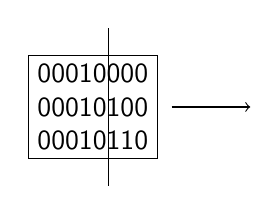
\begin{tikzpicture}
\node[draw,align=left] at (0,0) {00010000\\ 00010100\\ 00010110};
\draw (0.2,-1) -- (0.2,1);
\draw [->] (1,0) -- (2,0);
\end{tikzpicture}
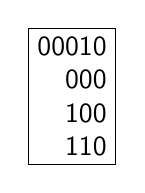
\begin{tikzpicture}
\node[draw,align=right] at (0,0) {00010\\ 000\\100\\110};
\end{tikzpicture}
\caption{The concept behind prefix sharing}
\label{fig:prefix-sharing}
\end{figure}

From the start on, the most important idea to speed up the reimplementation was to make use of \emph{prefix sharing}.
Imagine the left box in figure \ref{fig:prefix-sharing} represents a node which has some keys shown as bit strings.
All keys in the node have a prefix in common, so the same information is contained if we store the prefix and the additional bits (box on the right).
It is easy to see that less bits have to be stored now and therefore more keys can be packed on a page.
However, prefix sharing entails a lot of changes to the operations of the B+ tree. 
Because the prefix, and specifically its length, depends on the actual keys in a node, the maximum number of entries is different for every node.
This means that prefix sharing also affects all rebalancing operations.


\section{Implementation}
\subsection{Class Diagram} % (fold)
\label{sub:class_diagram}

For the new implementation of the index we have focused on achieving a balance between good design and code that offers good performance. Figure \ref{fig:class-diagram} show the class diagram for ZooDB.  
\begin{figure}[ht]
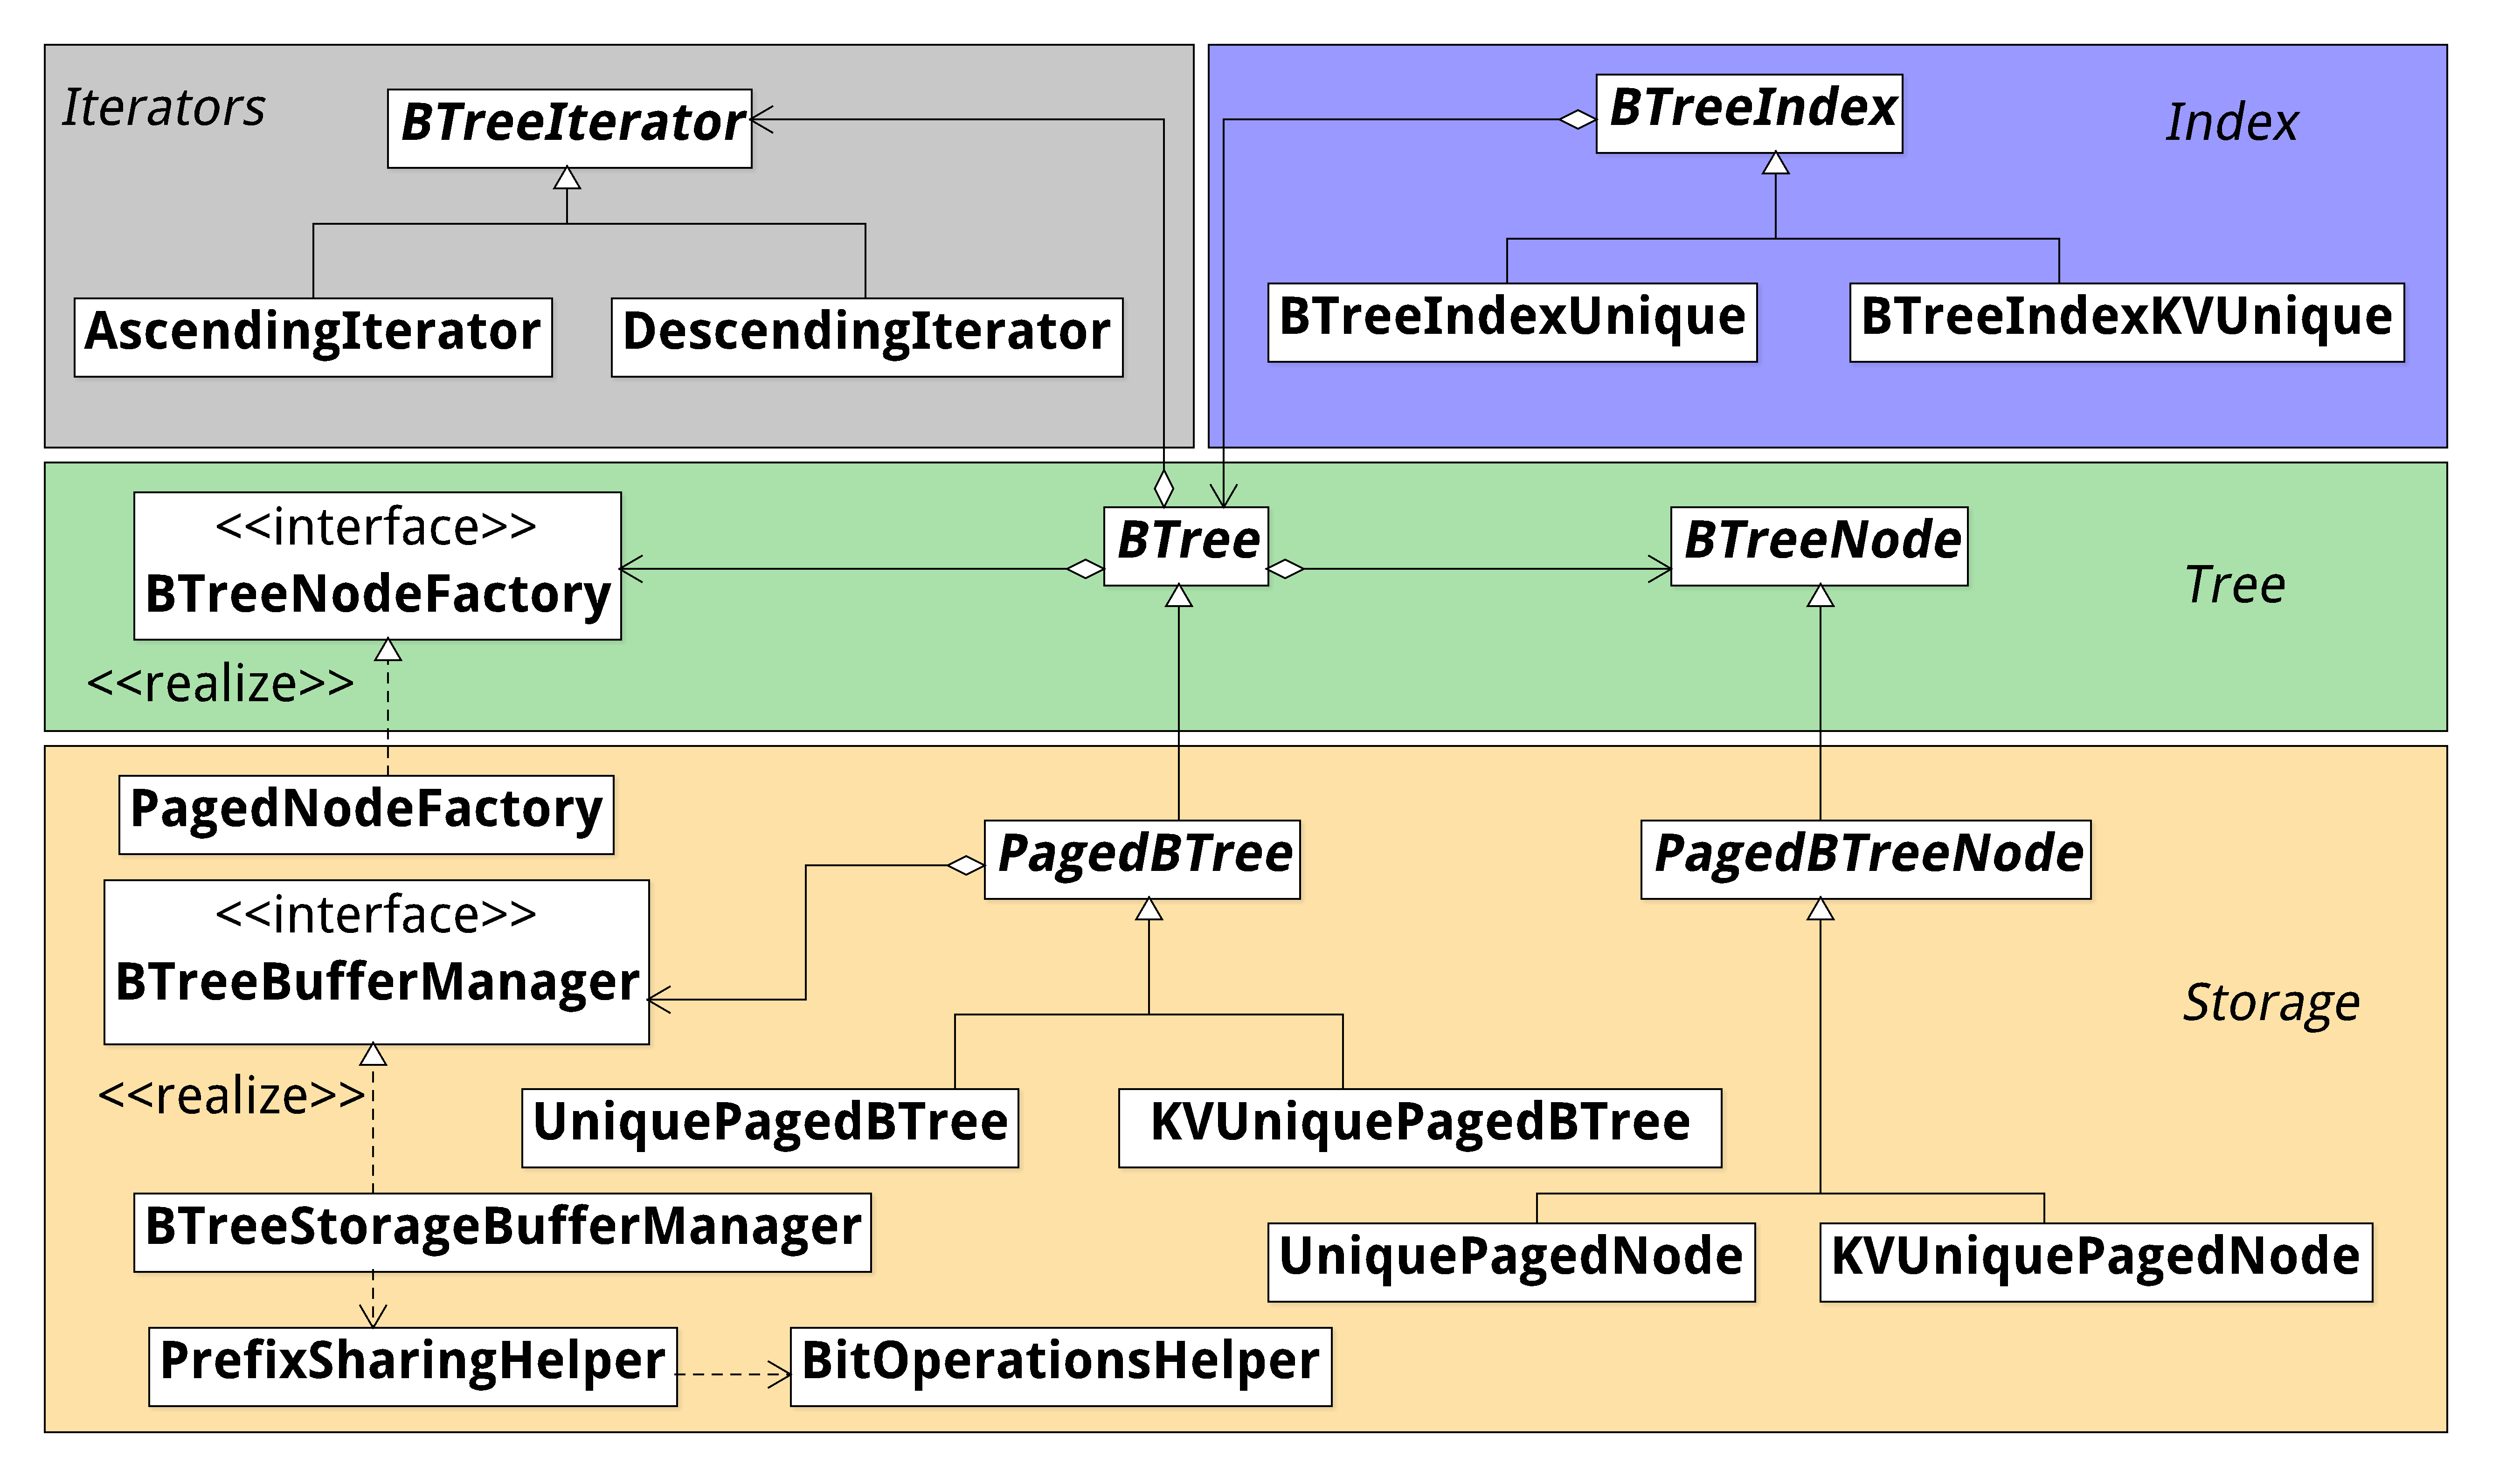
\includegraphics[scale=0.089, center]{ZooDBClassDiagram} 
\caption{The class diagram for the new index implementation}
\label{fig:class-diagram}
\end{figure}

% subsection subsection_name (end)
The \textbf{BTree} class implements all the logic for the B+ tree operations, including the re-balancing operations. The operations implemented operate on instances of the \textbf{BTreeNode} class. The \textbf{BTreeNode} abstract class contains the logic for a B+ tree node. To reduce the usage of polymorphism, we have opted not to implement different classes for leaf, inner or root nodes. The \textbf{BTreeNode} class has additional boolean fields, \textit{isLeaf} and \textit{isRoot} that are used to describe the position of a node within the tree. This choice reduces the size of the inheritance hierarchy, however in the cases where leaf nodes have to be treated differently than inner nodes we have added additional if statements to separate the behavior. 

The \textbf{BTreeNode} class holds no information about the child nodes of the node. However, this class exposes a number of abstract child access methods, like \textit{getChild()} or \textit{getChildren()}. These methods are implemented by the \textbf{PagedBTreeNode} class. Additionally, the \textbf{BTreeNode} class does not hold any information to differentiate between nodes belonging to unique and non-unique trees. All of the methods of for the \textbf{BTree} and \textbf{BTreeNode} classes which need to have different behaviour for unique and non-unique trees are abstract methods and will be overridden by the \textbf{UniquePagedBTreeNode} and \textbf{NonUniquePagedBTreeNode} classes.

The \textbf{PagedBTreeNode} holds the logic responsible for loading nodes from storage. class extends the \textbf{BTreeNode} and contains a reference to the \textbf{BufferManager} associated with the tree. Each instance of \textbf{PagedBTreeNode} contains a \textit{pageId}, which is given assigned by the \textbf{BufferManager} upon storage. The \textbf{PagedBTree} node contains information about the children of a node. We have opted to store the an array consisting of the page ids of the child nodes, instead of an array of hard references to the PagedBTreeNodes. Instead we store an array of weak references to the \textbf{PagedBTreeNode} objects. When a new node is loaded from disk, the child array is populated with the page ids of its child nodes while the array of weak references to the children is initialized to an array of null references. The first access to a child node will retrieve the \textbf{PagedBTreeNode} instance from the \textbf{BufferManager} and populate the weak references corresponding to its page id. Subsequent accesses to the child will use the weak reference, provided the child objects is not reclaimed by the garbage collector. If any of the children nodes are reclaimed by the garbage collector, they will be retrieved from storage on the next access and the weak reference will be repopulated.

The \textbf{UniquePagedBTreeNode} and \textbf{NonUniquePagedBTreeNode} classes extend the \textbf{PagedBTreeNode} class and contain data and behaviour specific to nodes belonging to unique and non-unique trees. For example, in case the non-unique nodes, inner nodes cotains the both a key array and a value array. This leads to different behaviour for unique and non-unique nodes during operations like peforming binary searches, shifting node entries to the left or right or copying node entries from one node to the other. This different behaviour is implemented in the aforementioned classes: \textbf{UniquePagedBTreeNode} and \textbf{NonUniquePagedBTreeNode}. 

The tree iterators are implemented by the \textbf{AscendingBTreeLeafEntryIterator} and \textbf{DescendingBTreeLeafEntryIterator} classes. The shared behaviour for these classes is implemented in the abstract class \textbf{BTreeLeafEntryIterator}. Because we have opted not to store information about the parent nodes, neither in the form of page ids or references, the iteration process requires the use of a stack to store the current position in the tree. The iterators do not support \textbf{Copy on Write} and are invalidated when the B+ tree is modified. 

The indexes are implemented in the \textbf{UniqueBTreeIndex} and \textbf{NonUniqueBTreeIndex} classes. As the index interface offers both methods to modify the B+ tree and to create iterators, we have opted to separate the tree logic in \textbf{BTree} and the iterator in \textbf{BTreeLeafEntryIterator}. This means that index objects delete all B+ tree operations to a reference of a \textbf{BTree} and create instances of \textbf{BTreeLeafEntryIterator} as needed.

The prefix sharing logic has been implemented in the \textbf{PrefixSharingHelper} class. Operations like computing the prefix, encoding/decoding the key array using prefix sharing and the re-balancing computations are available as static methods. We have choses to keep all this logic static to avoid creating extra computational objects that would have to be passed to \textbf{BTreeNode} objects upon creation.
% subsection class_diagram (end)

\subsection{Buffer Manager} % (fold)
\label{sub:buffer_manager}
The buffer manager is responsible for reading and writing \textbf{PagedBTreeNodes} to the \textbf{StorageChannel}.

The buffer manager instance is created in the constructor of a \textbf{BTreeIndex}. 
Its only direct function for the index is to ensure that all its content is written to disk when \texttt{write} is called on the index.

The buffer manager has two hash maps that map page ids to \textbf{PagedBTreeNode}s, one is for storing dirty (\texttt{dirtyBuffer}), 
the other for clean nodes (\texttt{cleanBuffer}). 
Using two hash maps allows to enforce a cache size on the \texttt{cleanBuffer} because its entries can be safely cleared.

The constructor of \textbf{PagedBTreeNode}s takes a \textbf{BufferManager} as argument and calls \texttt{save} on the buffer manager.
This advises the buffer manager to store the node in the \texttt{dirtyBuffer} with a negative id to indicate that this node has not been written yet.
If the index calls \texttt{write} on the buffer manager, it traverses through the tree, writes all dirty nodes to storage and marks them as clean.
During \texttt{write}, the buffer manager allocates a page, encodes a nodes data to a writable format and applies prefix sharing.

If a node's status changes from dirty to clean or vice versa, the node calls \texttt{updatePageStatus} on the buffer manager, 
which moves the node from the \texttt{dirtyBuffer} to the \texttt{cleanBuffer} or the other way round.

A \textbf{PagedBTreeNode} stores its children as an array of page ids, 
so the node needs the buffer manager to resolve page ids to actual \textbf{PagedBTreeNode} instances by calling the buffer manager's \texttt{read}.
Then the buffer manager tries to look up the page id in one of its memory buffers and if the page id is not in one of the memory buffers, the storage channel is queried.

Whenever a \textbf{PagedBTreeNode} is removed from the tree, it calls \texttt{close} on itself, which in turn calls \texttt{remove} on the buffer manager.
This instructs the buffer manager to delete the node from its memory buffers and to free the corresponding page.

\subsection{B+ Tree Operations} % (fold)
\label{sub:b_tree_operations}
One important implementation choice we have made is to store the key array unencoded in memory and to perform the prefix sharing encoding only when nodes are written to disk. While this approach increase the size of the node pages when loaded in memory, the advantage of this choice is that the costly key array encoding is only performed once, even if the node is modified multiple times before it is written to disk. 

Another advantage of having the key array unencoded in memory is that the search operations is similar to the search operation run on a traditional B+ tree. 

For the insert operation, if the new key has been inserted in the first or the last position of the key array, the prefix for the node has to be recomputed. The overflow is handled as follows:
\begin{enumerate}
	\item The algorithm first attempts to redistribute some keys from the current node to its left sibling. We do this to delay the moment when a new node is created. The exact redistribution process is described in the next section.
	\item If that is not possible, the current node is split into 2 nodes of equal size. One important different appears in how the new tree handles keys moving from one node to the other. In a traditional B+ tree, the max number of keys on a node is fixed, which makes it very to perform operations like splitting a node into 2 nodes of equal sizes. In case of prefix sharing, the first half of the keys could have a very different prefix size compared to the second half, which would lead to having 2 nodes with very different sizes. To avoid this, we perform a binary search to compute the optimal number of keys to move to the new node.
\end{enumerate}
	
In the case of the delete operation, the removal of an entry from the key array can cause the prefix to change. If the node from which the deletion has been performed is now underfull, a re-balancing procedure begin. The steps for the re-balancing are the following:
\begin{enumerate}
	\item In the first step, the algorithm first checks if the current node can be merged with \textbf{either} its left or its right neighbour. 
	\item If the merge at the previous step is not possible, the next step is to check whether the keys from the current node can be split between its left sibling \textbf{and} its right sibling. While this approach would involve in marking both the left and right siblings as dirty, the current node can then be removed.
	\item If the previous operation was not possible, some keys are redistribute from either the left or the right sibling. As a note, the success of the rebalancing operations is not guaranteed and the current node could remain underfull after the re-balance operation. However, we observed that this behaviour does not happen very often and does not have a significant impact on the tree size.
\end{enumerate}

% subsection b_tree_operations (end)

\subsection{Prefix Sharing Implementation} % (fold)
\label{sub:prefix_sharing_rebalancing}
When storing a node, the key array of a node is encoded into an array of bytes according to the common prefix. The encoding was performed at the bit-level, meaning that both the binary prefix and the deviations of elements from the prefix are computed as arbitrary number of bits. This means that if the binary prefix has length 9, it can be store in 2 bytes. Moreover, the remaining 7 bits from the second byte can be used to store part of the deviation of the fist array element. Other available alternatives for encoding would have been to compute both the prefix and the deviations as multiples of 8 and ensure that each encoded byte contains only prefix bits or deviation bits. We have chosen the bit-level encoding because it offers the best space reduction.

We have based the prefix sharing algorithms on the following observations about the binary prefix for an array of \textbf{sorted} integer elements.
\begin{itemize}
	\item The binary prefix of the array is equal to the binary prefix shared by the first and last element.
	\item Inserting a new element in the array in an ordered manner will either decrease the prefix of the whole array or leave it unchanged.
	\item Removing an element from the array will either increase the prefix of the whole array or leave it unchanged.
\end{itemize}

The main purpose of the split operation is to split the keys of a node that is overflowing between 2 nodes such that the node sizes are roughly the same. We perform this operation using a binary search to determine the optimal number of keys that have be moved from the current node such that the sizes of the current node and new node are as close as possible. The initial value for the number of keys to move is equal to half of the number of keys stored on the current node. The following logic is executed during each round of the binary search. 
\begin{enumerate}
	\item Compute the binary prefixes and sizes for the nodes that would result if the current number of keys k would be moved to a 
	new node. 
	\item Compute the different between the node sizes and if the current split is the best encountered so far, store the current number of keys to move and the size difference.
	\item If the size of the current node after the simulated key move is smaller than the size of the new node, decrease the number of keys to move. Otherwise, increase the number of keys to move.
\end{enumerate}
In the end, the split algorithm returns the number of keys to move corresponding to the minimum different in size between the current and new node.

A special case of the split operation is when the current node overflow and we would like to check if the key array can be equally split between the left and right siblings. In that case, the binary search is modified to search for number of keys to move to the right node, the remaining keys being moved to the left node. An additional optimization that we have added in that case is to stop at the first split that results in both left and right nodes having a valid size.

The goal of the redistribute operation is to move a number of keys from a node that is not underfull to an underfull node. It is desirable that at the end the split operation, neither of the nodes be underfull. If that is not possible, the redistribution fails and no keys are moved. The number of keys to move to the underfull node is computed in a similar manner to the split operation, using a binary search. Therefore, at each step, the prefixes and the sizes of the node that would result after the operation are computed. The binary search stops at the first split that results into two nodes of valid sizes.

The goal of the merge operation is reduce the number of nodes in the tree by merging an underfull node into either its left or right neighbours. In the case of the prefix sharing, the check that determines if two nodes can be merged is non-trivial, as it involves computing the prefix and the size of the node that would result after the merge. If the new node does not fit into a page file, the merge operation will not be performed.

% subsection prefix_sharing_rebalancing (end)

\section{Results}
\subsection{Microbenchmarks} % (fold)
\label{sub:microbenchmarks}
These microbenchmarks compare the old index and the reimplementation on artificial data. 
They in itself do not predict the performance of the whole database.
Each parameter configuration was rerun ten times. 
The page size was set to 4096 bytes.

Figure \ref{fig:unique_random_insert_numNodes} depicts the number of pages after inserting uniformly random entries in a unique tree.
It shows that prefix sharing does not give the desired reduction of size.
The probability of uniformly random entries having a long prefix is too small to achieve efficient encodings.
However, figure \ref{fig:unique_increasing_insert_numNodes} and \ref{fig:nonunique_random_insert_numNodes} demonstrate 
that when there is a good chance for a long prefix, the size of the tree is substantially smaller.
Increasing entries consist of incremental keys. The random entries for key-value unique indexes are copied 10 times to achieve duplication.
Naturally, incremental and duplicated keys are exploitable with prefix sharing.

On the other hand, figure \ref{fig:unique_increasing_insert} and \ref{fig:nonunique_random_insert} show that even in the best case inserting is slower with prefix-sharing.

Figure \ref{fig:unique_increasing_write} depicts the duration of writing the index after inserting. 
All nodes are dirty and have to be written.
Surprisingly, the saving in the number of nodes compensates for the duration of applying prefix sharing.

Figure \ref{fig:unique_increasing_search} shows that searching does not benefit from prefix-sharing. These search experiments were conducted by retrieving each key one after another.

To measure the performance of the remove operation we deleted $90\%$ of entries stored in the index.
Figure \ref{fig:unique_random_remove_numNodes} shows that the index reimplementation is balanced after removing. 
But proper rebalancing costs time (Figure \ref{fig:unique_increasing_remove}).

\begin{figure}
    \centering
    \makebox[0pt][c]{
      \begin{minipage}{0.3\textwidth}
      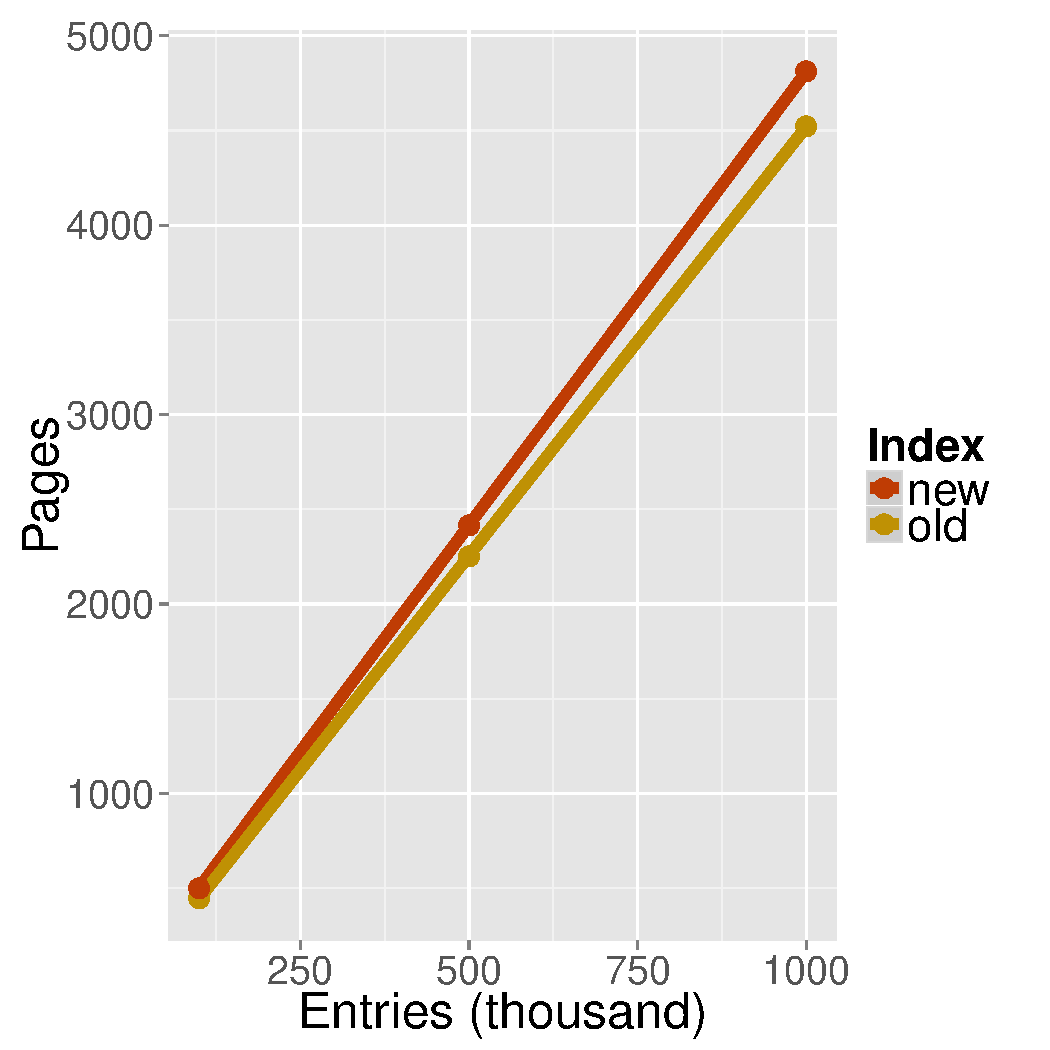
\includegraphics[scale=0.30]{images/unique_random_insert_numNodes.pdf} 
      \caption{Insert random entries in a key unique index.}
      \label{fig:unique_random_insert_numNodes}
      \end{minipage}
      \hspace{0.05\textwidth}
      \begin{minipage}{0.3\textwidth}
      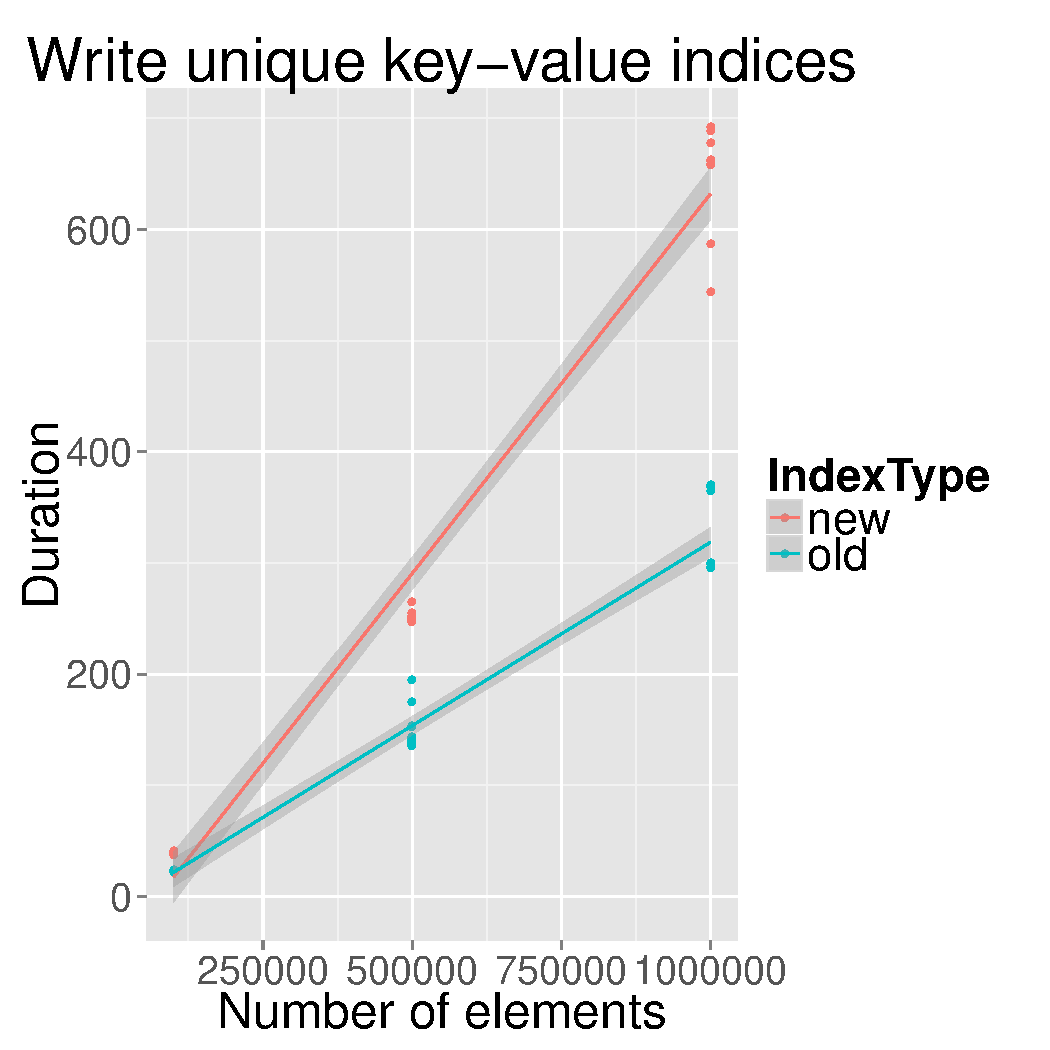
\includegraphics[scale=0.30]{images/unique_increasing_insert_numNodes.pdf} 
      \caption{Insert increasing entries in a key unique index.}
      \label{fig:unique_increasing_insert_numNodes}
      \end{minipage}
      \hspace{0.05\textwidth}
      \begin{minipage}{0.3\textwidth}
      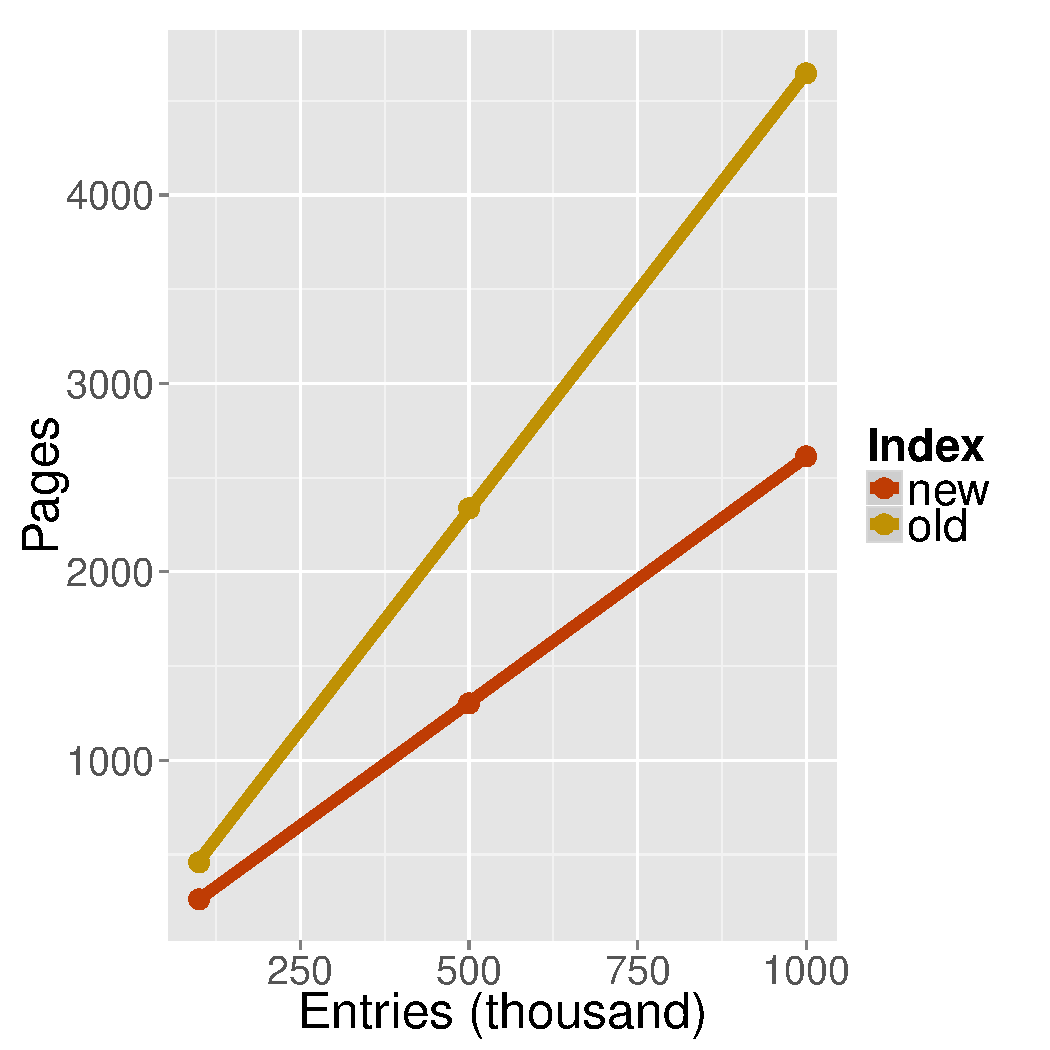
\includegraphics[scale=0.30]{images/nonunique_random_insert_numNodes.pdf} 
      \caption{Insert random entries in a key-value unique index.}
      \label{fig:nonunique_random_insert_numNodes}
      \end{minipage}
    }
\end{figure}
\begin{figure}
    \centering
    \makebox[0pt][c]{
      \begin{minipage}{0.3\textwidth}
      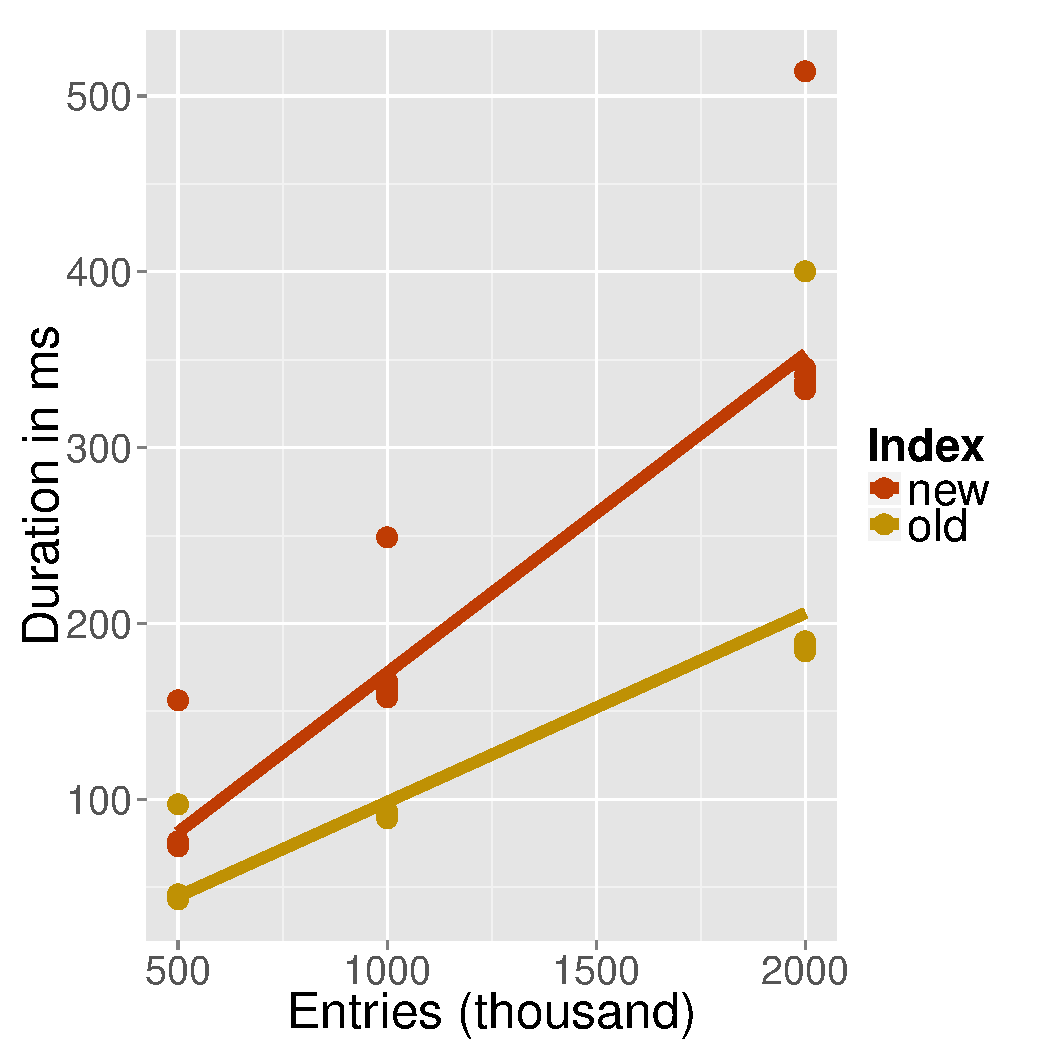
\includegraphics[scale=0.30]{images/unique_increasing_insert.pdf} 
      \caption{Insert increasing entries in a key unique index.}
      \label{fig:unique_increasing_insert}
      \end{minipage}
      \hspace{0.05\textwidth}
      \begin{minipage}{0.3\textwidth}
      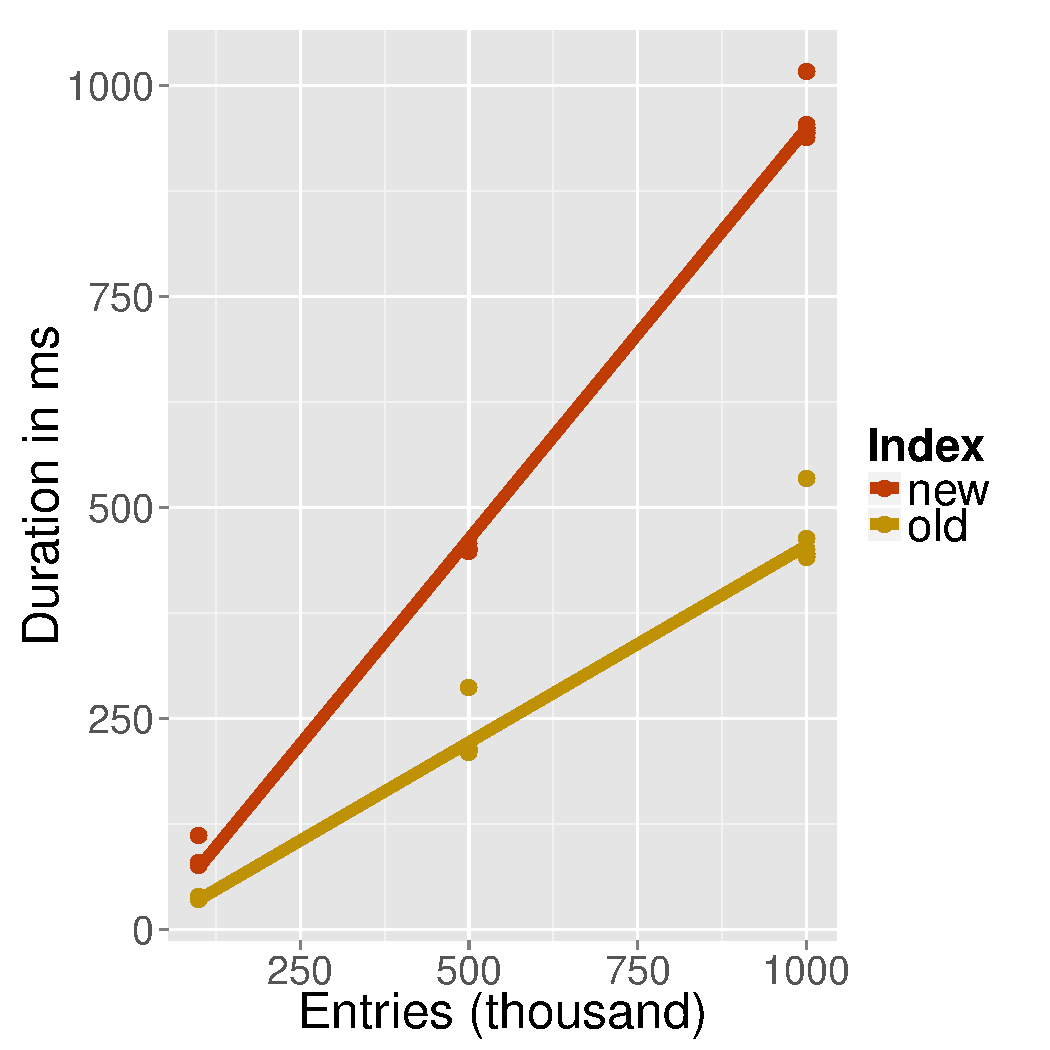
\includegraphics[scale=0.30]{images/nonunique_random_insert.pdf} 
      \caption{Insert random entries in a key-value unique index.}
      \label{fig:nonunique_random_insert}
      \end{minipage}
      \hspace{0.05\textwidth}
      \begin{minipage}{0.3\textwidth}
      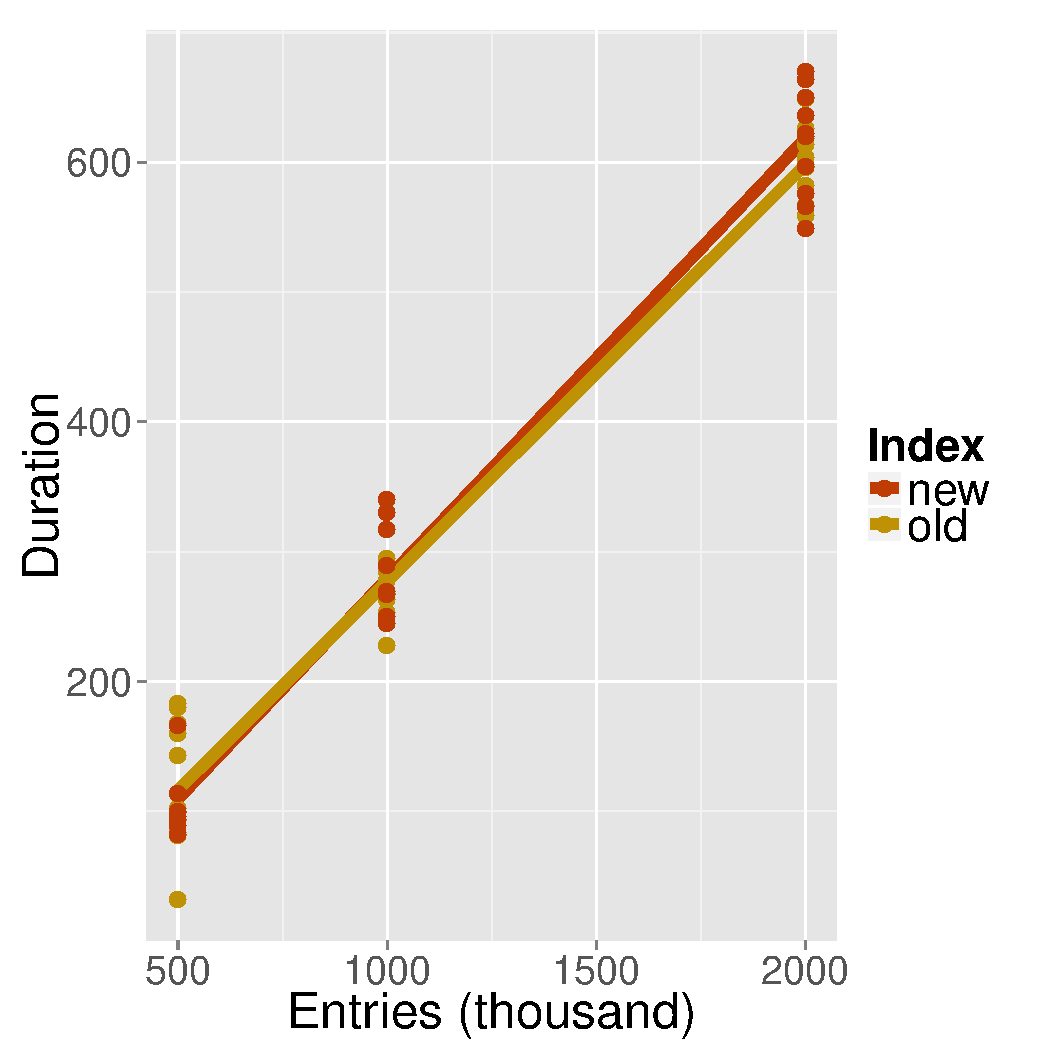
\includegraphics[scale=0.30]{images/unique_increasing_write.pdf} 
      \caption{Write after inserting increasing entries in a key unique index.}
      \label{fig:unique_increasing_write}
      \end{minipage}
    }
\end{figure}

\begin{figure}
    \centering
    \makebox[0pt][c]{
      \begin{minipage}{0.3\textwidth}
      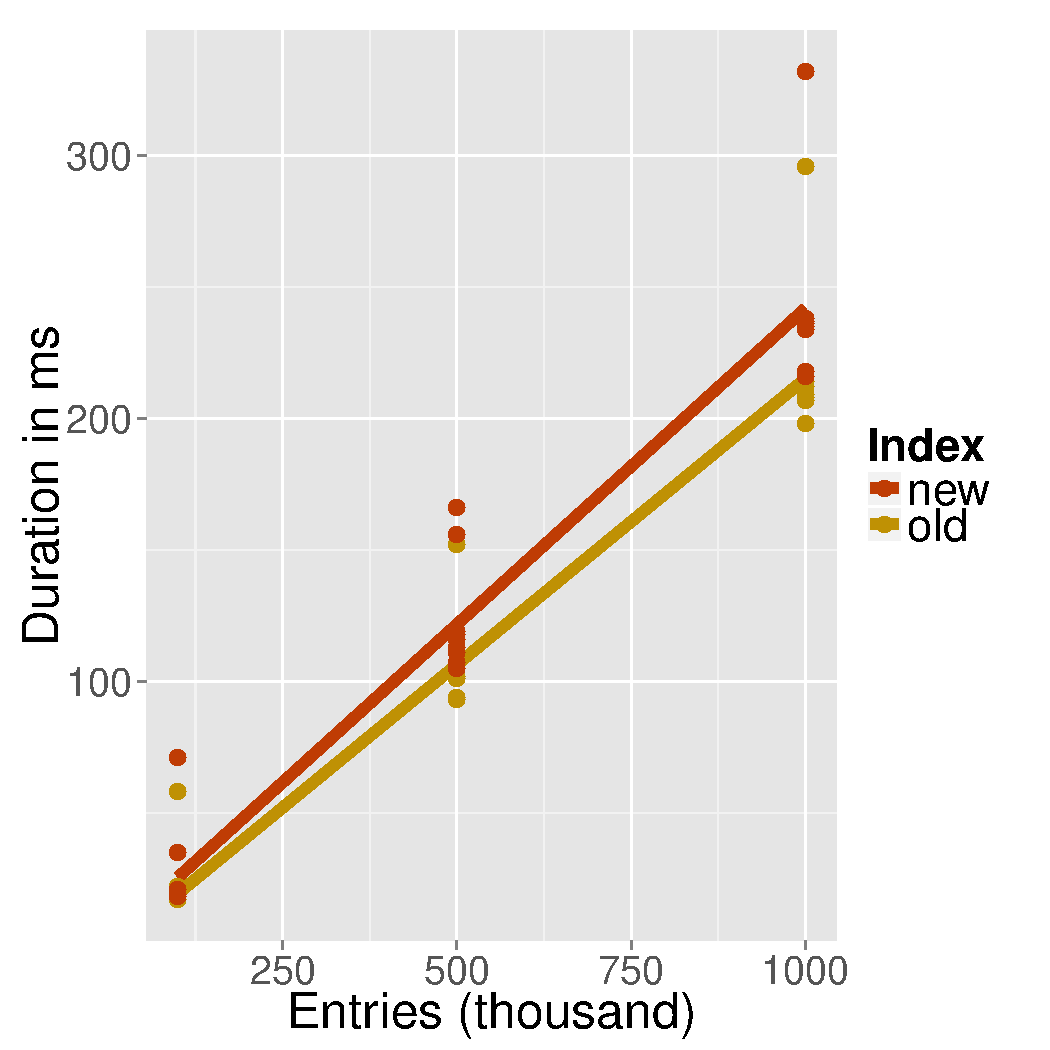
\includegraphics[scale=0.30]{images/unique_increasing_search.pdf} 
      \caption{Search increasing entries in a key unique index.}
      \label{fig:unique_increasing_search}
      \end{minipage}
      \hspace{0.05\textwidth}
      \begin{minipage}{0.3\textwidth}
      \centering
      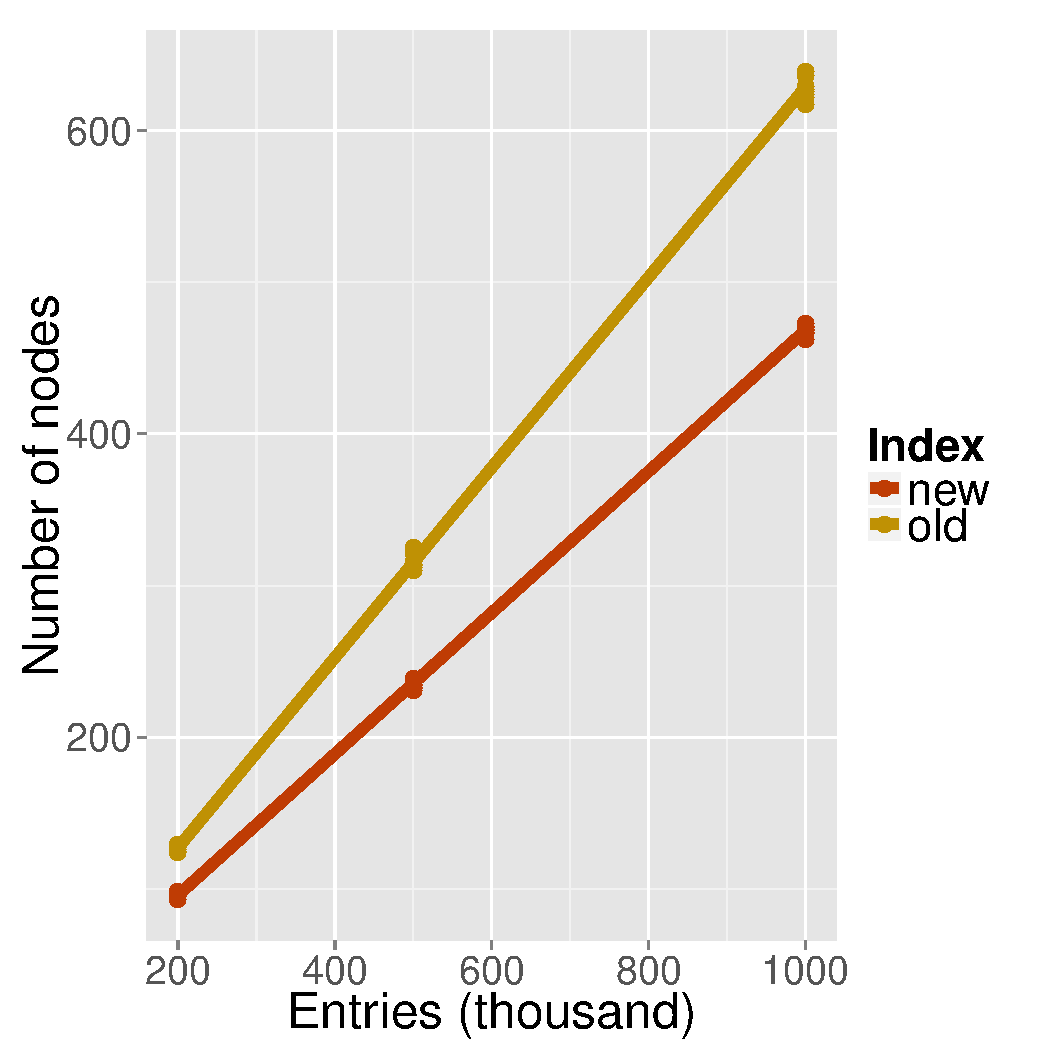
\includegraphics[scale=0.30]{images/unique_random_remove_numNodes.pdf} 
      \caption{Remove random entries from a key unique index.}
      \label{fig:unique_random_remove_numNodes}
      \end{minipage}
      \hspace{0.05\textwidth}
      \begin{minipage}{0.3\textwidth}
      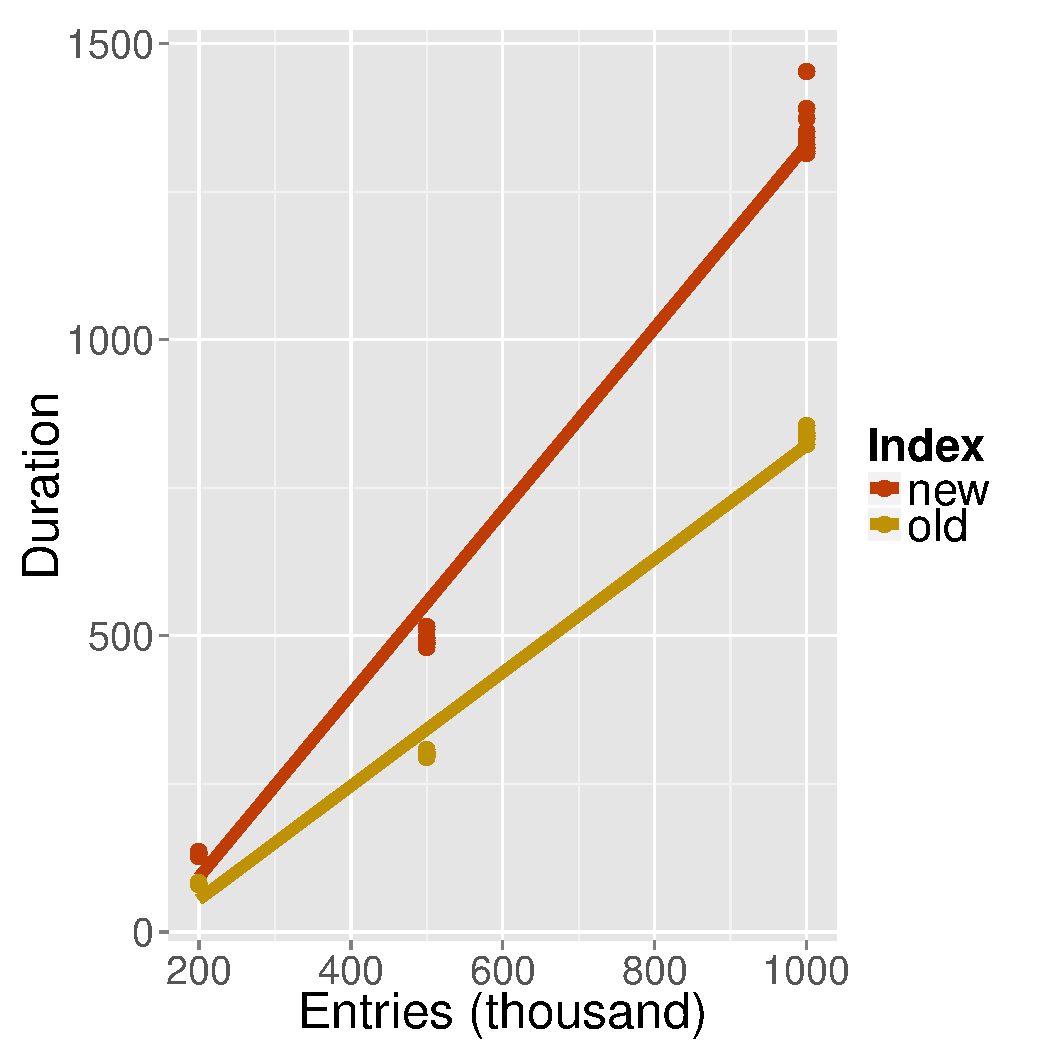
\includegraphics[scale=0.30]{images/unique_increasing_remove.pdf} 
      \caption{Remove increasing entries from a key unique index.}
      \label{fig:unique_increasing_remove}
      \end{minipage}
    }
\end{figure}

% subsection microbenchmarks (end)

\subsection{StackOverflow Import} % (fold)
\label{sub:stackoverflow_import}

\begin{figure}[h]
    \begin{minipage}{0.45\textwidth}
    \centering
	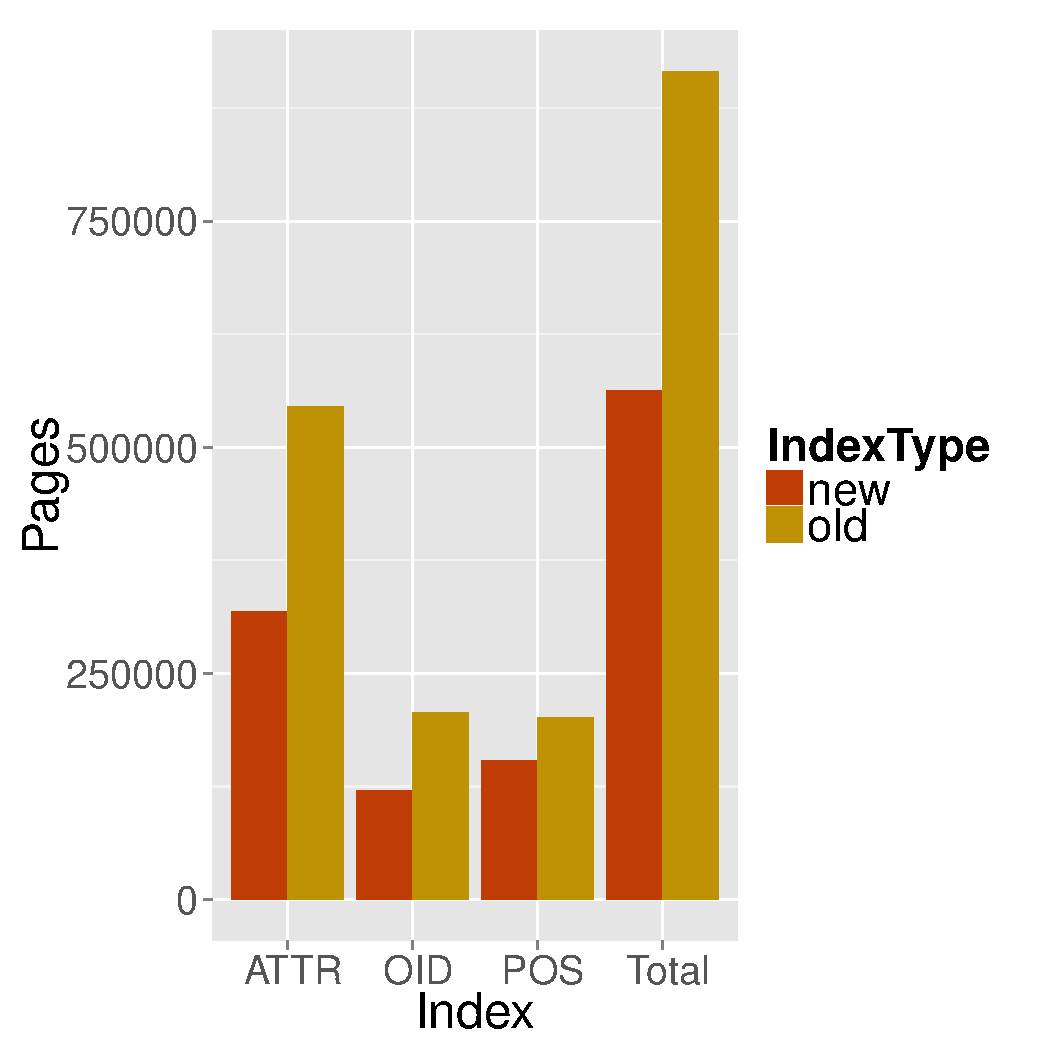
\includegraphics[scale=0.37]{images/SO_sizes.pdf} 	
	\caption{Comparison of number of index pages for the two index implementations}
	\label{fig:so-sizes}
	\end{minipage}
	\hspace{0.5cm}
	\begin{minipage}{0.45\textwidth}
	\centering
	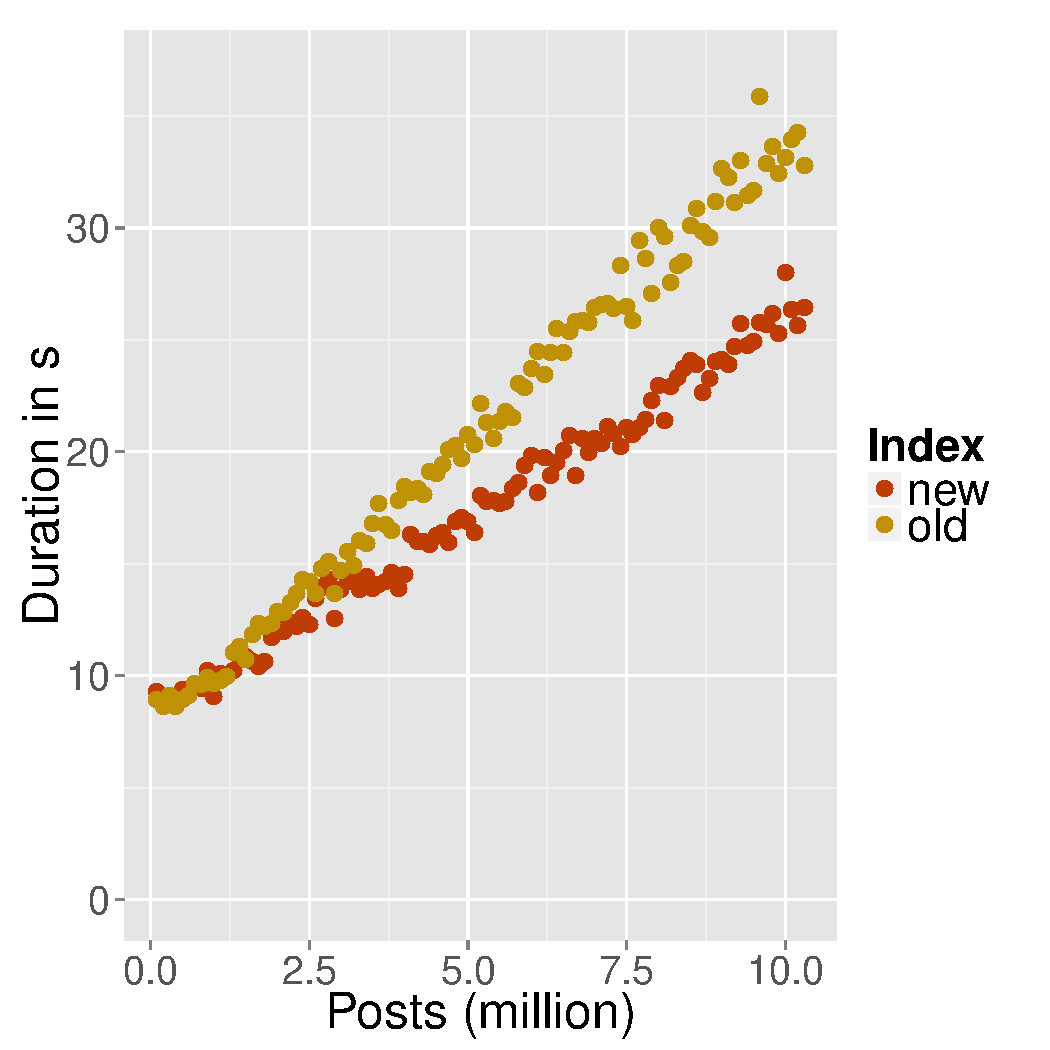
\includegraphics[scale=0.37]{images/SO_commit_duration.pdf} 
	\caption{Evolution of commit times for post objects}
	\label{fig:so-commits}
	\end{minipage}
\end{figure}

We have tested the performance of the new index implementation on a real world workload consisting of importing StackOverflow data from an XML dump. This data consisted of: 1.3 million users, 10.3 million posts, 13 million comments and 25 million votes. The attribute indexes that have been used for these objects were: 3 key unique indexes and 9 key-value unique indexes. The page size used was 4KB and the final database size was approximately 31 GB. 

Figure \ref{fig:so-sizes} shows the comparison between the number of index pages for different types of database indexes after the import operation was completed. The free space index is not included in the graph as it did not use the prefix sharing implementation. The attribute index was 41.6\% smaller, the OID index was 41.5\% small and the Position index was 23.1\% smaller. The total reduction of index pages was 38.5\%. 

Figure \ref{fig:so-commits} shows the evolution of the commit durations for post objects. Each point on the graph represents the commit of a batch of post objects. For each point, the distance on the horizontal axis represents the number of post objects already stored in the database, while the distance on the vertical axis shows the commit duration. One can notice that for both indices, the commit duration increase as the number of posts that are already stored increases. However, the prefix sharing index presents a slower increase, as the commit times are generally smaller than the commit times for the old index implementation. 

Moreover, the total duration of the import with the new index implementation was 25\% smaller than the duration of the import with the old index. The main reason for this difference is that the number of pages writes is smaller for the new index implementation. As the number of entries stored on a page increases, there is a higher probability that all writes in a transaction are restricted to a smaller number of pages, especially since the data accesses in a database respect a certain data locality.
% subsection stackoverflow_import (end)
% section results (end)

\section{Summary} % (fold)
\label{sec:summary}

The report has presented the new index implementation for ZooDB. The main additions in the new implementation are the Buffer Manager and the encoding of the keys using the shared binary prefix. The Buffer Manager Prefix abstracts the access to disk pages and can be configured as a cache of arbitrary size. Prefix sharing offers a trade-off between the speed of index update operations, like insert and delete, and the space saved as a result of packing more key-value entries into a single node. The microbenchmarks show that each single index update operation is slower on the prefix-sharing index. However, the microbenchmarks do not properly predict the behaviour of the database using the new index, as the space savings offered by prefix sharing result in less page IO operations. Thus, the new index performs good in practice, especially in the case of larger databases, like the one resulted after the StackOverflow import.
% section summary (end)
\end{document}
